\chapter{Evaluation}
\section{Experimental Settings}
\subsubsection{Dataset Generation}

The training set is generated by rendering synthetic views of the object 3D models from uniformly sampled 2562 viewpoints, additionally with 36 in-plane rotations at each viewpoint, together $2562 \times 36 = 92232$ views. 
\\[8pt]
The test set is rendered from randomly sampled 1000 viewpoints on the sphere with random in-plane rotation, i.e. $1000 \times 1 = 1000$ views.
\subsubsection{Dataset Augmentation}
While keeping reconstruction targets clean, following random augmentations are applied to the input images: 
(\romannumeral 1) applying random cropping, translation and resizing; 
(\romannumeral 2) varying image contrast, brightness and color distortions;
(\romannumeral 3) inserting random background images from Lorem Picsum dataset \cite{Picsum}. 


\subsubsection{Training Settings}
During the training of the autoencoder, I used the Adam optimizer with a learning rate of $2 \times 10^{-4}$, a batch size $= 64$..

\newpage
\section{Experimental Results}
\subsection{Visualization of the Training Process}
\begin{figure}[H]
	\subfigure[pitcher base]{
		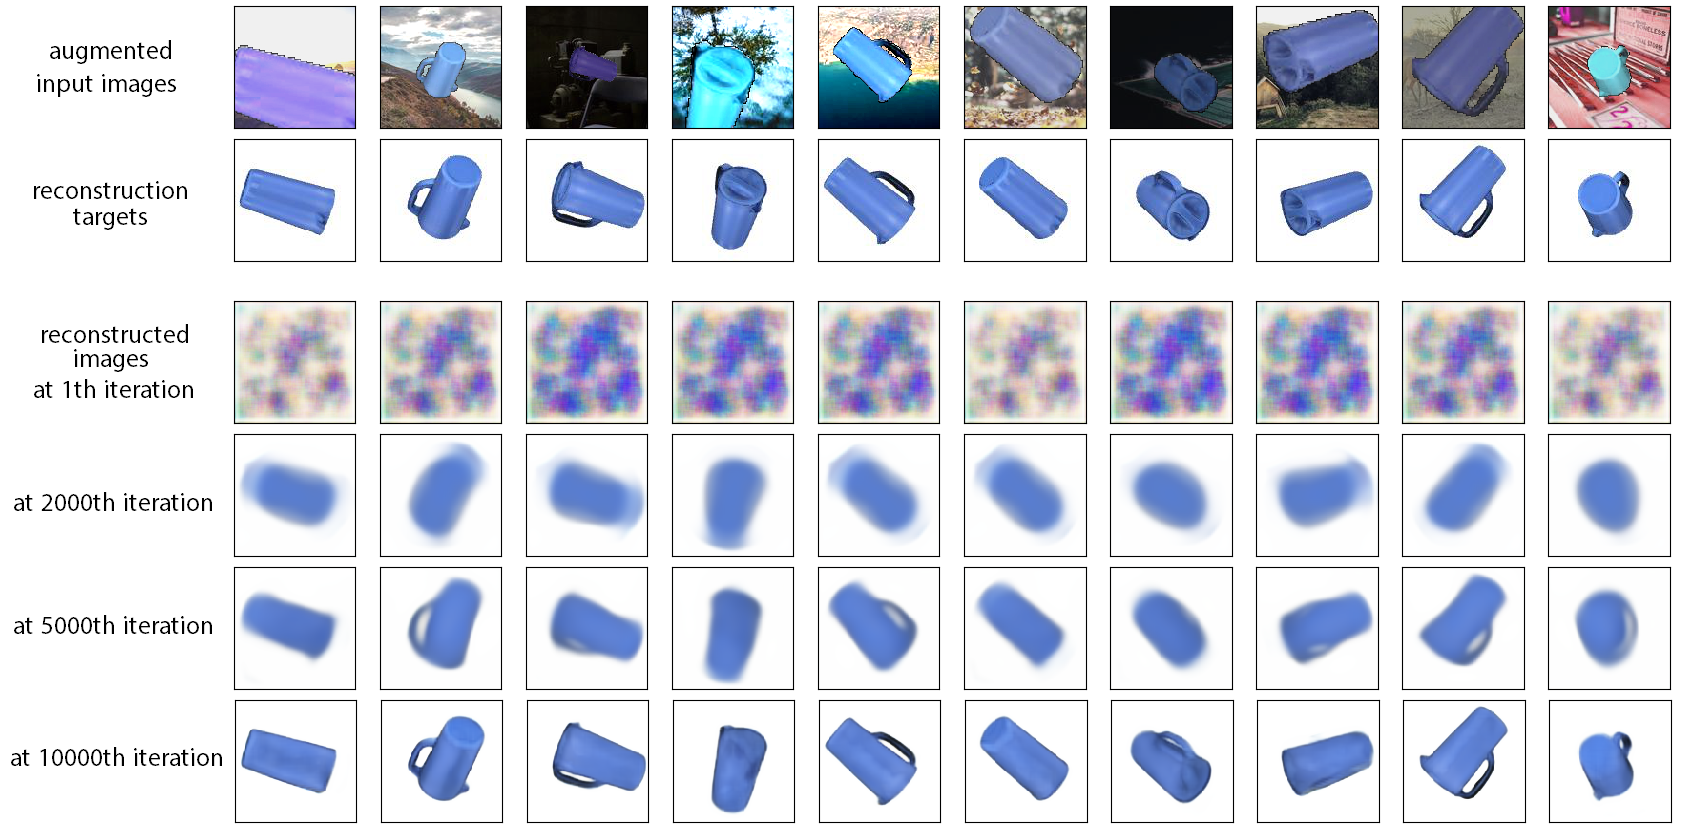
\includegraphics[width=1.05\textwidth]{trainingprocess}
		\label{fig:regular}
	}
	\subfigure[bowl]{
		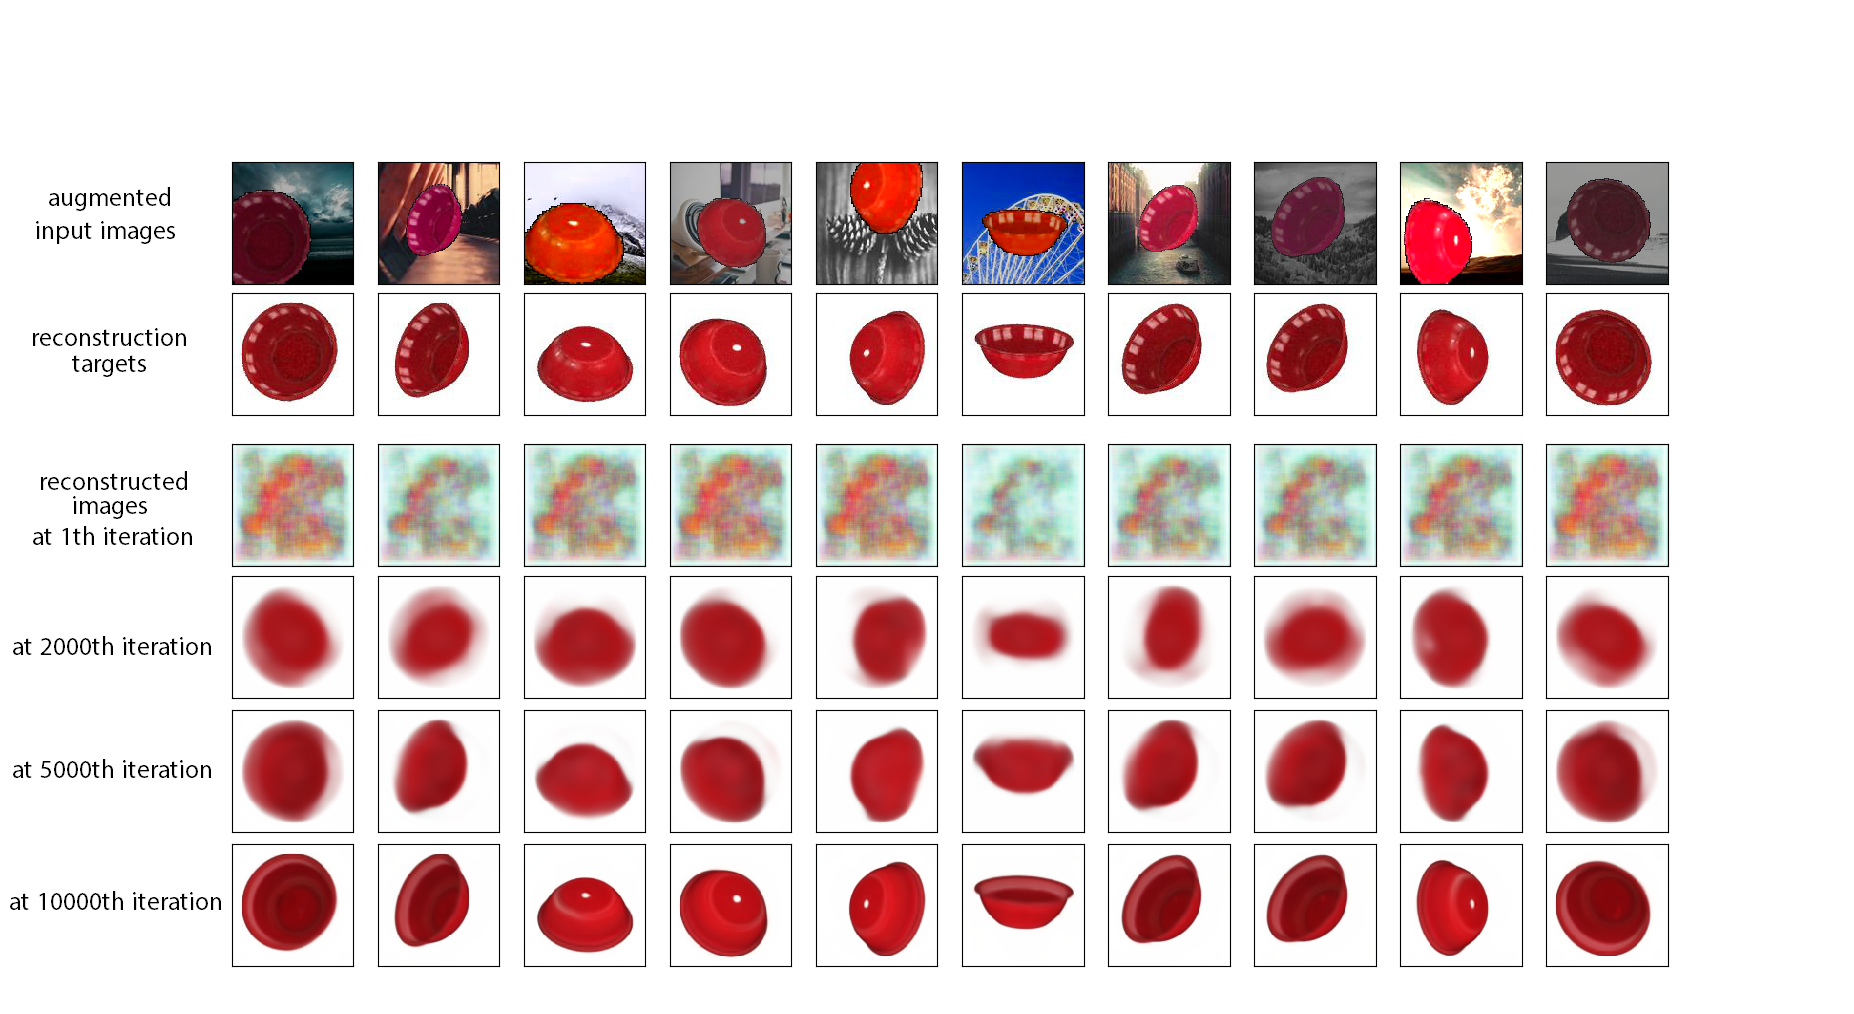
\includegraphics[width=1.15\textwidth]{bowl}
		\label{fig:random}
	}
	\caption[Visualization of the training process]{\textbf{Visualization of the training process}}
	\label{fig:trainingprocess}
\end{figure}


As shown in Fig. \ref{fig:trainingprocess}, the reconstructed images are randomly initialized at the beginning of the training. After around 2000 iterations, the autoencoder is able to extract a vague shape of the object. With the training time going by, the quality of the reconstructed object images increase. After around 10000 iterations, the orientation and the structure of the object can be very good reconstructed.

\subsection{Rotation error}
In order to evaluate the pose estimation results, the rotation error $\theta_{err} $ between the ground truth and the estimated rotation matrix of the object is computed via \ref{eq:error1} and \ref{eq:error2}: 
\begin{align}
	R_{err} = R_1 \cdot R_2^T
	\label{eq:error1} \\	
	\theta_{err} = arccos(\frac{tr(R_{err})-1}{2})
	\label{eq:error2}	
\end{align}


\setlength{\tabcolsep}{20pt}
\renewcommand{\arraystretch}{1.5}
\begin{tabular}{|m{5.5cm} | m{3.0cm}| m{3.0cm}|}

	\hline
	\multicolumn{3}{|c|}{unsymmetrical object (pitcher base)} \\
	\hline
	\diagbox{test set}{training set} &augmented &non-augmented \\
	\hline
	augmented    &0.09796& 2.47153  \\
	\hline
	non-augmented  &0.05773    &0.05556\\
	\hline
	\multicolumn{3}{|c|}{unsymmetrical object (bowl)} \\
	\hline
	\diagbox{test set}{training set} &augmented &non-augmented \\
	\hline
	augmented &0.50277 & 2.18787 \\
	\hline
	 non-augmented &0.12769&  0.22125\\
\hline
\end{tabular}
 \begin{center}
 	Table 3.1: \textbf{Rotation error [radian] between ground truth and estimated pose in different scenarios}
 \end{center}
\vspace{4pt}
The test errors in different scenarios are reported in table 3.1. Based on the testing results, we can come to the following conclusions:\\[8pt] (\romannumeral 1) Because of the pose ambiguities, the rotation error tested on the symmetrical object is larger than unsymmetrical objects. Nevertheless, the orientation of symmetrical objects can still be good extracted as shown in Fig. \ref{fig:trainingprocess}. \\[8pt]
(\romannumeral 2) The autoencoder trained on the non-augmented training set performs very well on the non-augmented testing set. However, it fails to generalize to the augmented dataset.\\[8pt]
(\romannumeral 3) The autoencoder trained on the augmented training set is able to achieve a good performance both on the augmented and on the non-augmented dataset.